\chapter{基于深度学习的个性化推荐}
信息过载时代的到来推动了推荐系统的兴起与发展,海量数据的积累也引发了深度学习的热潮。
鉴于深度学习在诸多研究领域的成功应用和突破性进展,近些年来,如何将深度学习成功应用于推荐系统领域中成为了研究者们的热门话题。
本章节中,我们首先使用神经网络中传统的多层感知器(Multilayer Perceptron, MLP)对求解推荐问题进行初步探索,
取得了和经典推荐算法相近的实验效果,证明了深度学习在推荐系统中应用的可行性;
然后考虑到用户兴趣随时间流逝产生漂移的现象,本文提出了长短期兴趣模型(Long Short Interest Model, LSIM)
来刻画用户的长期兴趣和短期兴趣,利用区域性的神经网络结构对时序信息进行提取,进一步提升了推荐性能。
下面我们就来详细介绍这些基于深度学习的个性化推荐算法。

\section{电影评分预测任务}
\begin{figure}[htbp]
\centering
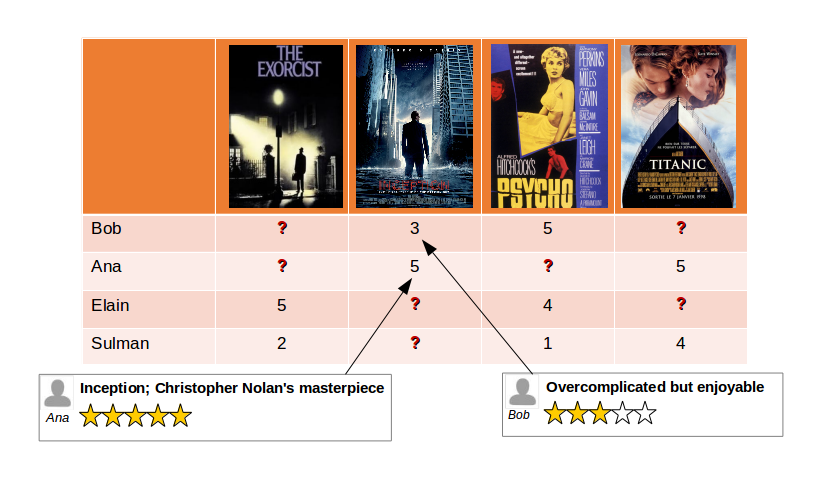
\includegraphics[scale=0.6]{images/task1.png}
\caption{电影评分预测任务中的稀疏矩阵}
\label{fig:task1}
\end{figure}

现实生活中,推荐系统的具体应用场景繁多,被推荐的对象也是各式各样,例如商品推荐、音乐推荐、电影推荐、论文推荐等等。
推荐系统研究领域中,为了便于研究各类推荐算法,研究者提出了一系列的推荐评测任务,其中最为著名的就是电影评分预测任务。
特别地,2006年举办的Netflix百万美金大奖赛也是采用的该评测任务。
该评测任务在数学形式上可以表达为,在电影推荐平台上存在着$\mathbf{N}$位用户和$\mathbf{M}$部电影,
同时用户在使用的过程中会产生一定数量的评分数据,评分$\mathbf{r}_{ij}$代表第$i$位用户给第$j$部电影的评分数据,
数值的高低表明了用户对该部电影的兴趣程度。相对于整个电影集合而言,用户通常只会评价其中的一小部分,
因此这些评分数据构成了一个巨大的稀疏矩阵$\mathbf{R} \in \mathbb{R}^{N \times M}$,
里面包含已观察到的评分和待预测的评分,推荐算法的目标就是根据已观察到的评分建模用户和电影之间的相互关系,
并以之去预测那些待预测的评分,最后我们可以将具有较高预测分的且用户没有观看过的电影推荐给用户。

图\ref{fig:task1}给出的电影评分预测任务中的稀疏矩阵样例,其中包含Bob、Ana、Elain和Sulman$4$个用户,
《The Exorcist》、《Inception》、《Psycho》和《Titanic》$4$部电影,以及已观察到的$9$个评分,
这些评分数据构成了一个$4 \times 4$的稀疏评分矩阵。已观察到的评分在图中以黑色数字显示,评分的范围是$1$分到$5$分,
$1$分代表用户对该部电影的不满意,$5$分代表用户非常喜爱该部电影,而待预测的评分在图中以红色问号的形式展示。
推荐系统研究者需要设计推荐算法对用户和电影之间的关系进行建模,预测出这些待评测的评分数据,并且向相关用户进行相应的电影推荐。

\begin{figure}[htbp]
\centering
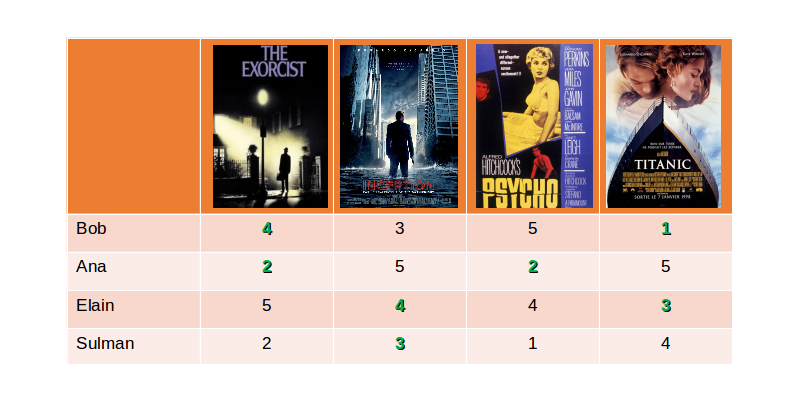
\includegraphics[scale=0.6]{images/task2.png}
\caption{电影评分预测任务中的预测矩阵}
\label{fig:task2}
\end{figure}

图\ref{fig:task2}给出的电影评分预测任务中的预测矩阵样例,是推荐系统研究者通过推荐算预测出来的评分矩阵,
其中绿色的评分即当初需要进行预测的待评分数据。在图中我们可以观察到推荐算法预测出用户Bob可能给电影《The Exorcist》评价$5$分,
说明电影《The Exorcist》非常符合用户Bob的兴趣爱好;同时推荐算法还预测出用户Bob可能给电影《Titanic》评价$1$分,
说明用户Bob不是很喜爱《Titanic》的电影风格。所以我们可以将电影《The Exorcist》推送到用户Bob的推荐列表中,
帮助用户Bob发现他可能喜爱的电影,从而完成整个推荐过程。

\section{基于多层感知机的推荐}
\subsection{多层感知机}
多层感知器是一种基于前馈人工神经网络的分类器,图\ref{fig:mlp}展示了一个最基本的三层结构的多层感知器,
其中Input代表输入层,研究者可以将样本信息通过该层输入到多层感知器中;Hidden代表隐藏层,
通过全连接的边结构和激活函数从输入层学习出更高层次的抽象表示;Output代表输出层,利用多分类函数将抽象表示映射到训练目标上。

\begin{figure}[htbp]
\centering
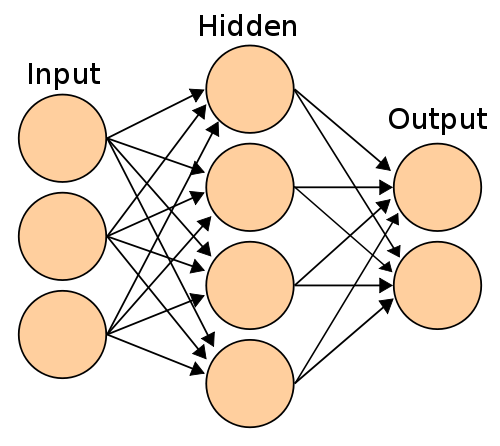
\includegraphics[scale=0.4]{images/mlp.png}
\caption{多层感知器模型}
\label{fig:mlp}
\end{figure}

多层感知器中的每一层的神经节点,可以理解为对上一层特征表示的更高层次的抽象表示,多层感知器通过一层层的抽象,
将原始输入一步步映射到训练目标上去。假设第$i$层包含$n$个神经节点,构成一个长度为$n$的特征向量$l_i$,
第$i+1$层包含$m$个神经节点,构成一个长度为$m$的特征向量$l_{i+1}$,那么两者通过如下公式进行映射:

\begin{equation}
l_{i+1} = \sigma( W_i l_i + b_i )
\end{equation}

其中$W_i$是大小为$m \times n$的权值矩阵,$b_i$是长度为$m$的偏移向量,$\sigma$函数是非线性的激活函数,
常见的$\sigma$函数包括Sigmoid函数、Tanh函数和ReLU函数等。多层感知器一般采用误差反向传播算法进行训练。

\subsection{UM模型}
电影评分预测问题中,每一个训练样本包含三类信息:用户ID、电影ID和评分数据,需要我们设计模型从用户ID和电影ID出发,
在训练数据中发现两者之间的相互联系,预测出评分数据。本文利用多层感知器设计如下图所示的网络结构去建模用户电影关系。

\begin{figure}[htbp]
\centering
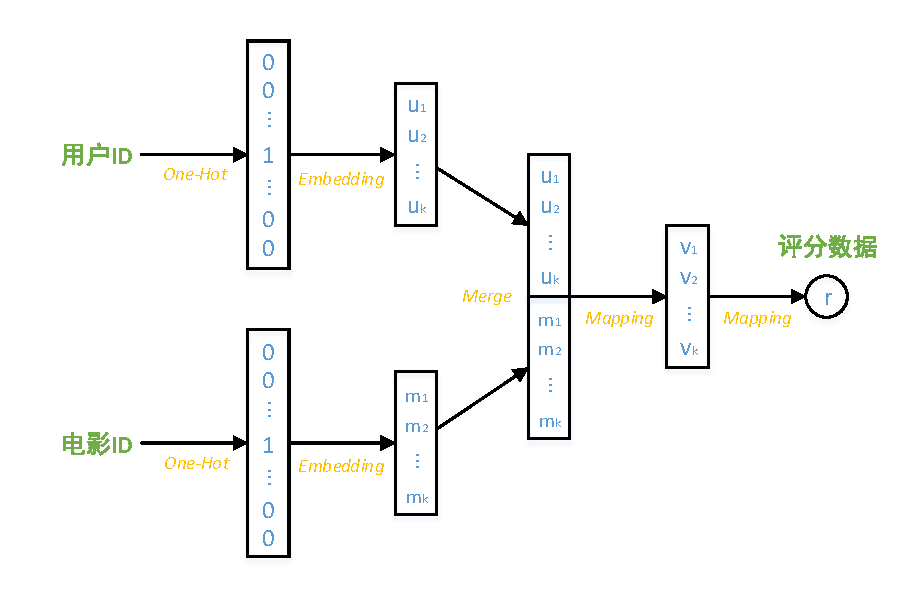
\includegraphics[scale=0.7]{images/a_b.pdf}
\caption{基于多层感知器的UM模型}
\label{fig:a_b}
\end{figure}

图\ref{fig:a_b}中展示的是本文提出的第一个神经网络模型,我们将其标记为UM模型,其中符号U代表用户User,符号M代表电影Movie。
在UM模型中,我们接受用户ID和电影ID作为输入,首先使用独热表示将其数字向量化,例如对于用户ID为$1$的用户,一共存在$100$个用户,
那么该用户ID就会向量化成一个长度为$100$的向量,向量的第$1$位元素的数值为$1$,其他元素的数值都为$0$。

一般来说,一个真实的推荐平台中存在大量的用户和电影,所以独热向量都具有较大的维度,不宜直接作为神经网络中的节点。
因此我们使用嵌入(Embedding)技术将维度较高的独热向量映射到低维的嵌入向量。嵌入技术使用嵌入矩阵实现,
嵌入矩阵的行数对应用户数量,列数对应低维特征向量维度,嵌入技术将独热表示向量和嵌入矩阵相乘,得到嵌入向量,
等价于把用户在嵌入矩阵中对应的行向量进行取出。

在经过读热表示和嵌入化后,得到了低维的用户嵌入向量和电影嵌入向量,紧接着我们将两者进行拼接,输入到多层感知器的输入层中,
经历若干隐藏层的抽象提取后,将预测评分数据在输出层进行输出。在UM模型中,我们将预测准确率作为我们的训练目标,
因此具体的损失函数为:

\begin{equation}
\ell = \sum{ (r - \hat{r})^2 }
\end{equation}

其中$r$代表真实的评分数据,$\hat{r}$代表多层感知器的预测评分数据,UM模型需要在所有训练样本上最小化真实评分和预测评分之间的差距。

\subsection{U-M模型}
UM模型直接将用户嵌入向量和电影嵌入向量作为输入加入到多层感知器中,通过隐藏层学习两者之间的相互联系。
通过多层感知器学习出来的用户嵌入向量和电影嵌入向量可以看成是一种兴趣分布,每一个维度对应到对某一方面的感兴趣程度。
可以这样理解,如果用户兴趣分布和电影兴趣分布较为类似,则说明该部电影比较符合用户的口味;相反,
如果用户兴趣分布和电影兴趣分布相差较大,则说明用户可能不是很喜爱观看该部电影。

\begin{figure}[htbp]
\centering
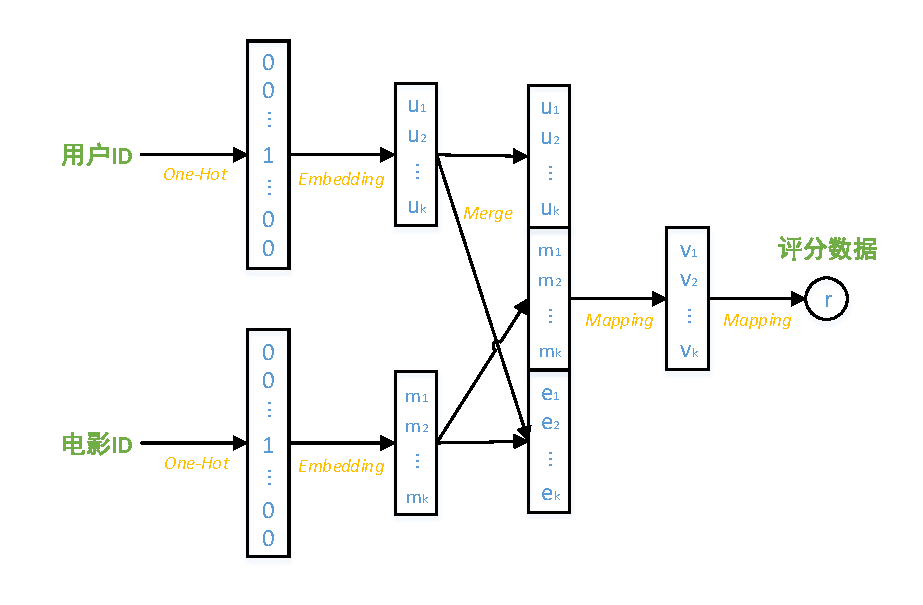
\includegraphics[scale=0.7]{images/a_b_a-b.pdf}
\caption{基于多层感知器的U-M模型}
\label{fig:a_b_a-b}
\end{figure}

考虑到以上分析,本文引出了差值向量的概念,在数值上,差值向量等价于将用户嵌入向量和电影嵌入向量进行相减;
在概念上,差值向量体现了用户兴趣分布和电影兴趣分布的差异情况。同时,我们将差值向量也作为输入引入到UM模型中,
形成了如同图\ref{fig:a_b_a-b}所示的模型框架。和UM模型的不同之处在于,在连接用户嵌入向量和电影嵌入向量进行输入的同时,
额外连接了两者的差值向量:

\begin{equation}
\vec{e}_i = \vec{u}_i - \vec{m}_i \quad , \quad i \in (1,2,...,k)
\end{equation}

其中$\vec{u}$和$\vec{m}$是用户和电影对应的嵌入向量,$\vec{e}$是两者的差值向量。
我们将该模型标记为U-M模型,其中符号U代表用户User,符号M代表电影Movie,符号-代表差值的含义。

\subsection{Dropout技术}
本文在多层感知器的训练过程中同时也采用了Dropout技术,可以帮助模型得到具有更高鲁棒性的训练。
Dropout技术首先被Hintion等人\parencite{hinton2012improving}提出,是神经网络模型在训练过程中的一种trick操作。
具体而言,Dropout技术在神经网络训练的过程中,以移除概率$p$虽然让网络中的某些隐藏层的节点的权重不工作,
这些不工作的界面可以蚕食认为不是网络结构的一部分,但实际上的权重是被保存在节点中的,只是不被误差反向传播算法更新而已,
直到下一次没有被选中为不工作节点,它就又可以进行权重传播了。在预测过程中,不存在不工作节点,可以理解为移除概率$p=0$。

\begin{figure}[htbp]
\centering
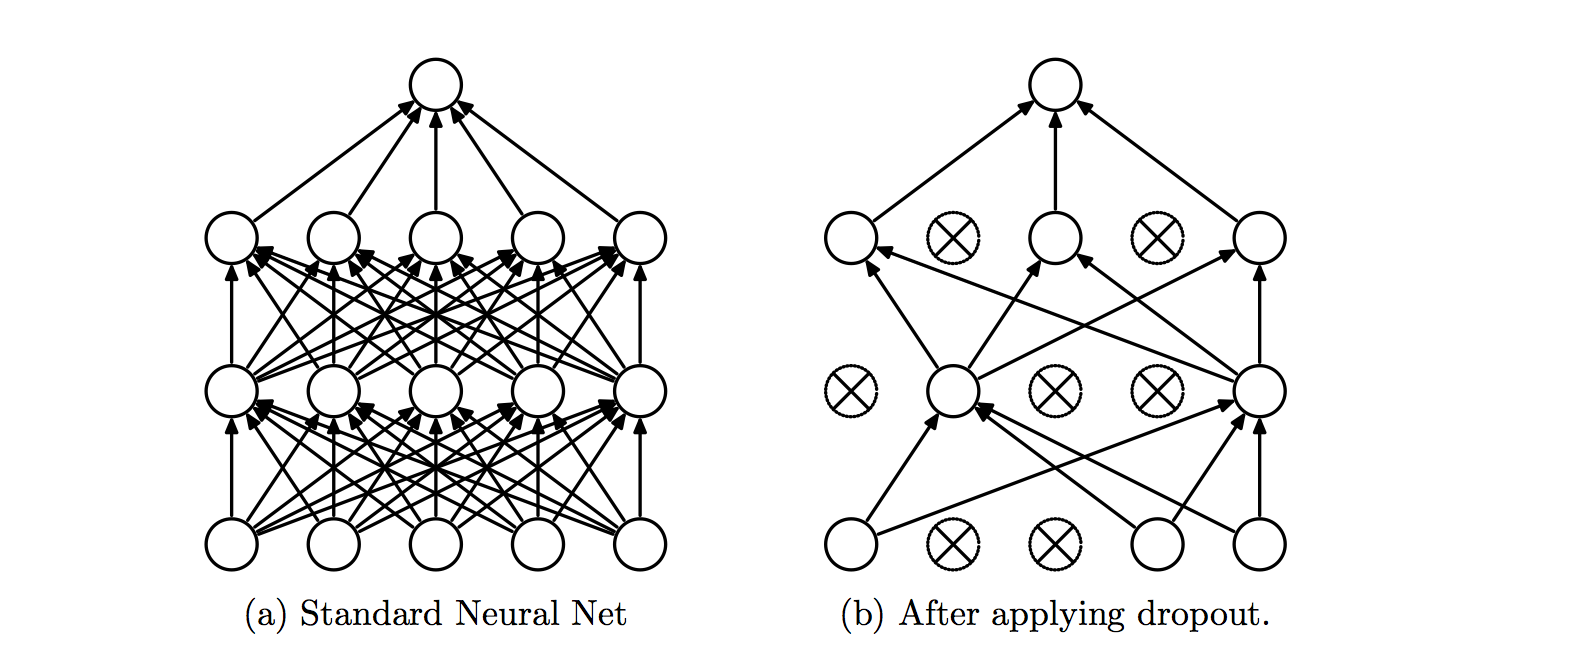
\includegraphics[scale=0.5]{images/dropout.png}
\caption{Dropout技术}
\label{fig:dropout}
\end{figure}

图\ref{fig:dropout}展示了应用Dropout技术前后的神经网络结构图,左半部分是原始的多层感知器模型,每一层的隐藏节点和下一层的隐藏节点是全连接的,
右半部分是采用Dropout技术后的多层感知器模型,每一层都有一定比例的隐藏节点被移除,成为了原模型的一个子结构。
Dropout技术可以看作成模型平均的一种。对于每次输入到网络中的样本而言,因为不工作节点的分布是随机的,其对应的网络结构也就是不同的。
但所有的这些不同的网络结构又同时共享了隐含节点的权值,是的不同样本可以对应到不同的模型中,和集成学习中Bagging技术的一种特殊情况。

\section{基于长短期兴趣模型的推荐}
\subsection{长期兴趣和短期兴趣}
协同过滤算法是推荐系统中应用最广泛的算法之一,成功解决Netflix百万美金大奖赛后,备受学术界和工业界的研究和投入。
协同过滤算法的基础假设是被同一用户偏爱的诸多物品具有相似的兴趣分布,或者喜欢相同物品的诸多用户拥有相似的兴趣分布。
然而在现实的环境中,由于用户的兴趣会随着时间发生变化(学术上称之为兴趣漂移现象),这样的假设并不总是成立。

\begin{figure}[htbp]
\centering
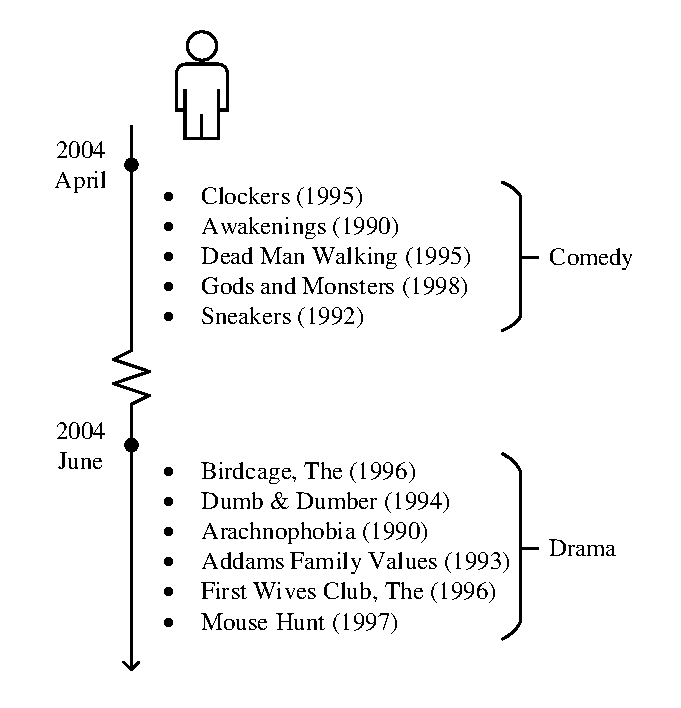
\includegraphics[scale=0.7]{images/example.pdf}
\caption{数据集MovieLens-1M中ID号为$5988$的用户的观影时间线}
\label{fig:example}
\end{figure}

例如,对于著名推荐系统数据集MovieLens-1M中一名ID号为$5988$的用户,我们将他的电影评分数据按照时间进行排序,
构成了图\ref{fig:example}所展示的观影时间线。从图中我们可以观察得到,该用户在2004年四月份的时候热衷于观看喜剧类电影,
然后在2004年六月份开始转为喜爱观看戏剧类电影。同时我们还可以发现,对于指定的用户,在一个固定的时间段内,
该用户的兴趣分布往往是稳定的,不会发生剧烈的变化。为了描述这种现象,本文提出了两个定义:长期兴趣和短期兴趣,
它们的具体描述如下:

\begin{enumerate}
\item \textbf{长期兴趣} 反映了用户在整个时间区间上的兴趣分布,它体现在用户在整个时间区间上所有喜爱和讨厌的物品的整体集成上。
\item \textbf{短期兴趣} 反映了用户在某一固定时间子区间上的兴趣分布,它体现在用户在这个固定时间子区间上所有喜爱和讨厌的物体的整体集成上。
\end{enumerate}

从两者的定义可以推理出,一个用户可以拥有一个长期兴趣和若干个短期兴趣。在图\ref{fig:example}的例子中,
ID号为$5988$的用户的长期兴趣就是既喜爱观看喜剧类电影又喜爱观看戏剧类电影,同时该用户又拥有两个短期兴趣,
分别是四月份的喜爱观看喜剧类电影,和六月份喜爱观看戏剧类电影。

\subsection{带时序特征的基础假设}
从上文中的长期兴趣和短期兴趣的定义上可以看出,传统的协同过滤算法只考虑了用户的长期兴趣,
即使在用户较长间隔时间观看的两部电影属性类别差别很大,它们也会在算法层面上被等同视之。
短期兴趣却可以从更细的角度出发,描述用户和电影之间的相互联系,以及用户兴趣随时间发生的种种变化。

长期兴趣体现在整个时间区间中交互过的物品上,而短期兴趣则体现在若干时间子区间中交互过的物品上,
并且随着时间的推移不断发生变化,为了体现短时间兴趣分布的特点,本文提出了带时序特征的基础假设:
首先,对于同一个长期兴趣中的若干短期兴趣,处于相同短期兴趣中的那些电影的相似度应该大于处于不同短期兴趣的电影;
其次,对于不同的长期兴趣中的若干短期兴趣,电影之间的相似度应该和它们出现在相同短期兴趣的次数呈正相关关系,
如果出现次数越多,电影之间的相似度也会越高,出现次数越少,电影之间的相似度也越低。

\begin{figure}[htbp]
\centering
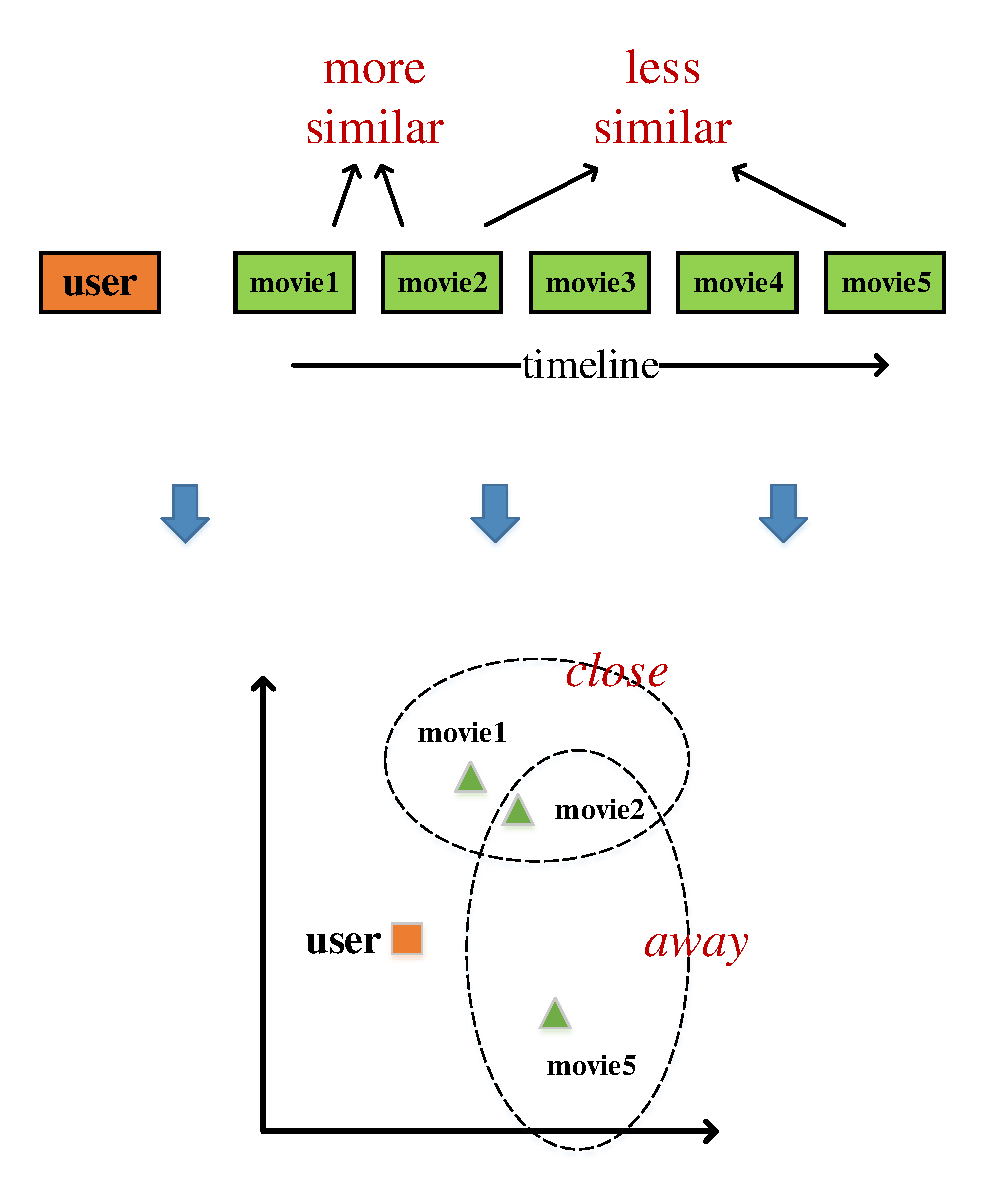
\includegraphics[scale=0.5]{images/embedding.pdf}
\caption{电影之间的相似度在低秩嵌入空间中的表现}
\label{fig:embedding}
\end{figure}

为了体现带时序特征的基础假设,本文使用嵌入技术将用户和电影映射到低秩向量空间中,电影之间的相似度即可转化为对应向量之间的空间距离。
以图\ref{fig:embedding}为例,在图的上半部分中展示了一位用户的观影时间线,为了方便演示,其中只包含了$5$部电影,
并且按照观影时间进行了排序。如果假定短期兴趣的范围为两部电影,而且各个短期兴趣之间可以存在交集,那么在该观影时间线中就拥有$4$个短期兴趣,
分别是<$item1$,$item2$>,<$item2$,$item3$>,<$item3$,$item4$>和<$item4$,$item5$>。
拿电影$item2$为例,它和电影$item1$处于同一个短期兴趣中,而和电影$item5$处于不同的短期兴趣中,
那么电影$item2$和电影$item1$的相似度应该大于和电影$item5$的相似度。
通过嵌入技术我们分别将用户和电影映射到低秩嵌入空间内,在图的下半部分,我们给出了在低秩嵌入空间中三者的空间位置,
电影之间的相似度可以通过向量之间的距离展示,在图中可以明显看出向量$item2$和$item1$之间的距离小于和向量$item5$之间的距离。

\subsection{观影时间线 V.S. 语句模型}
通过上文中提到的带时序特征的基础假设,我们发现电影评分预测任务中的用户观影时间线和自然语言处理任务中的语句模型十分类似。
如图\ref{fig:example2}所示,图的上半部分是某一用户的观影时间线,包含$8$部电影,下半部分则是一个语句模型,拥有$10$个词语。
观影时间线上的用户可以对应到语句模型中的句子本身,它们都有一个带有某种顺序关系的序列;而一部部电影可以对应到一个个词语,
它们的共同点在于符合彼此相对距离和相似程度成反相关的趋势,即相对距离越近,相似程度越高,反之相对距离越远,相似程度越低。

\begin{figure}[htbp]
\centering
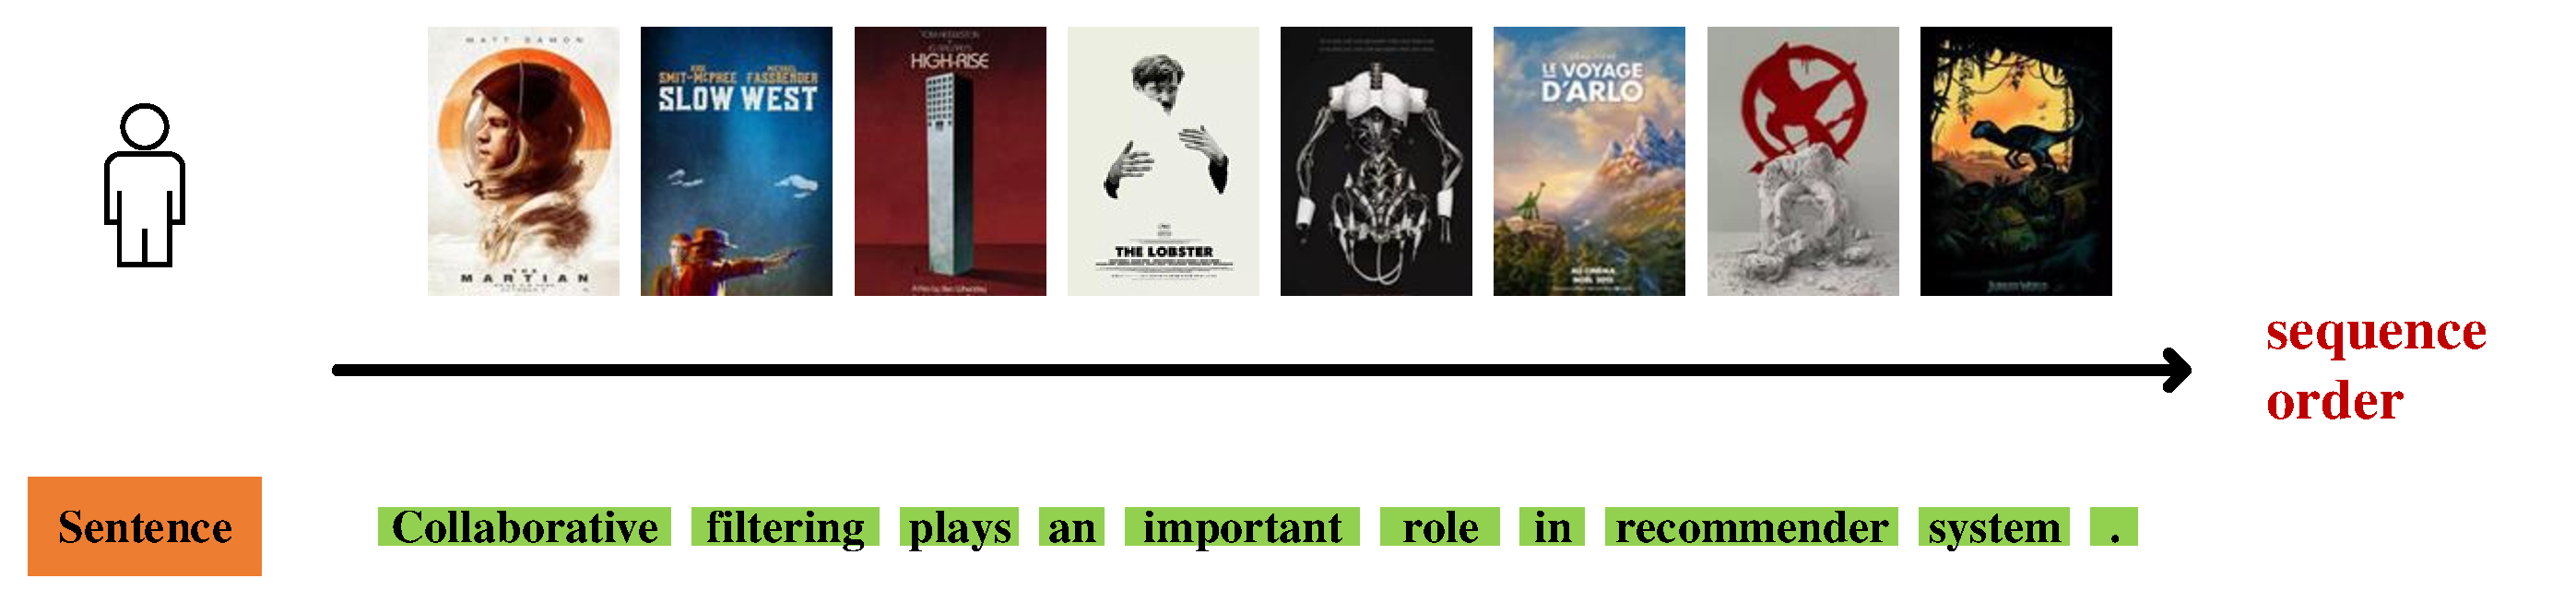
\includegraphics[scale=0.33]{images/example2.pdf}
\caption{电影时间线 V.S. 语句模型刻}
\label{fig:example2}
\end{figure}

自然语言处理Paragraph2Vec算法\parencite{le2014distributed}在经典Word2Vec算法的基础上,加入了句子向量作为一个全局的上下文信息,
同时学习词语嵌入表示的同时学习出整个句子的嵌入表示,这样可以避免在需要使用句子嵌入表示的时候,勉强使用词语嵌入表示求和或者求均值来代替的窘境,
在情感分类和信息检索任务上取得了较优的实验效果。受到该算法的启发以及观影时间线和语句模型的相似性,
本文提出了长短期兴趣模型LSIM,利用用户具有长期兴趣和短期兴趣的特点,
从用户的观影时间线中提取电影之间的序列信息,学习出更好的用户嵌入向量表示和电影嵌入向量表示。

\subsection{长短期兴趣模型}
本文提出的长短期兴趣模型是一个生成式模型,通过训练样本中的数据最大化其生成的概率,并且在此过程中顺便学习出用户嵌入向量和电影嵌入向量。
首先我们进行符号定义,假设电影推荐平台中存在$N$个用户$x_i(i \in 1,2,...,N)$以及$M$部电影$y_j(j \in 1,2,...,M)$
\footnote{我们使用符号$x$和$y$代替经典的$u$和$v$以避免符号$v$和向量符号$\mathbf{v}$在阅读上的误解},
每一位用户都拥有一个观影时间线$T_i(i \in 1,2,...,N)$,包含了按照时间排序的若干电影信息$y_{i_1}$, $y_{i_2}$, ..., $y_{i_{L_i}}$,
其中$L_i$代表用户$x_i$观影时间线上电影的数量,其数值远远小于电影数量$M$。

\subsubsection{用户生成}
\begin{figure}[htbp]
    \centering
    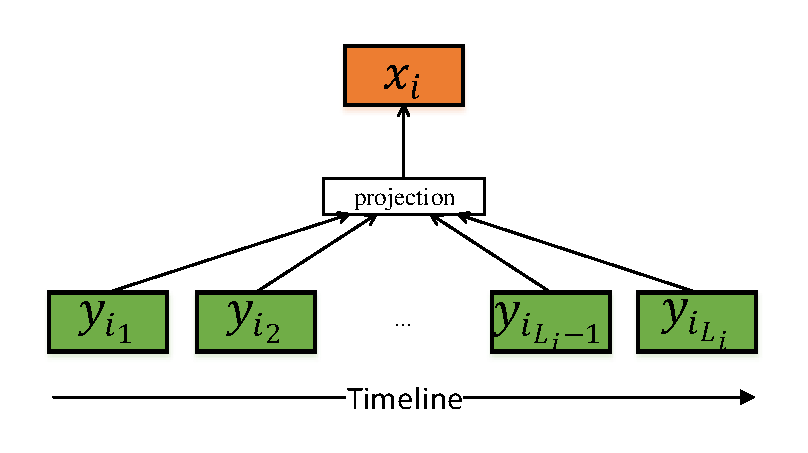
\includegraphics[scale=0.6]{images/doc2vec1.pdf}
    \caption{LSIM模型中的用户生成}
    \label{fig:doc2vec1}
\end{figure}

然后,对于每位用户的观影时间线,我们将其作为一个样本进行输入,在该样本中,我们需要依次生成用户和各部电影。
用户的生成过程如图\ref{fig:doc2vec1}所示,该过程可以看做成是用户长期兴趣的一种体现,
接收观影时间线上所有电影的输入,最终生成该用户,即

\begin{equation}
p(x_i | y_{i_1}, y_{i_2}, ..., y_{i_{L_i}}) =
\frac
{
    exp ( \overline{\mathbf{v}}_{1}^{\mathrm{T}} \mathbf{v}_{x_i}^{'} )
}
{
    \sum_{x^{'}} exp ( \overline{\mathbf{v}}_{1}^{\mathrm{T}} \mathbf{v}_{x^{'}}^{'} )
}
\end{equation}

其中$x^{'}$代表用户集合中的每一位用户,$x_i$代表当前待生成的用户,
$\mathbf{v}_{x^{'}}^{'}$和$\mathbf{v}_{x_i}^{'}$是分别是它们的输出向量表示,
整个公式的含义就是在当前观影时间线的前提下,当前用户的生成概率要大于其他用户的生成概率,
而$\overline{\mathbf{v}}_{1}$代表用户$x_i$的观影时间线上的所有电影的输入向量的平均值,即

\begin{equation}
\overline{\mathbf{v}}_{1} = \frac{\sum_{j=1}^{L_i} \mathbf{v}_{y_{i_j}}}{L_i}
\end{equation}

\subsubsection{电影生成}
\begin{figure}[htbp]
    \centering
    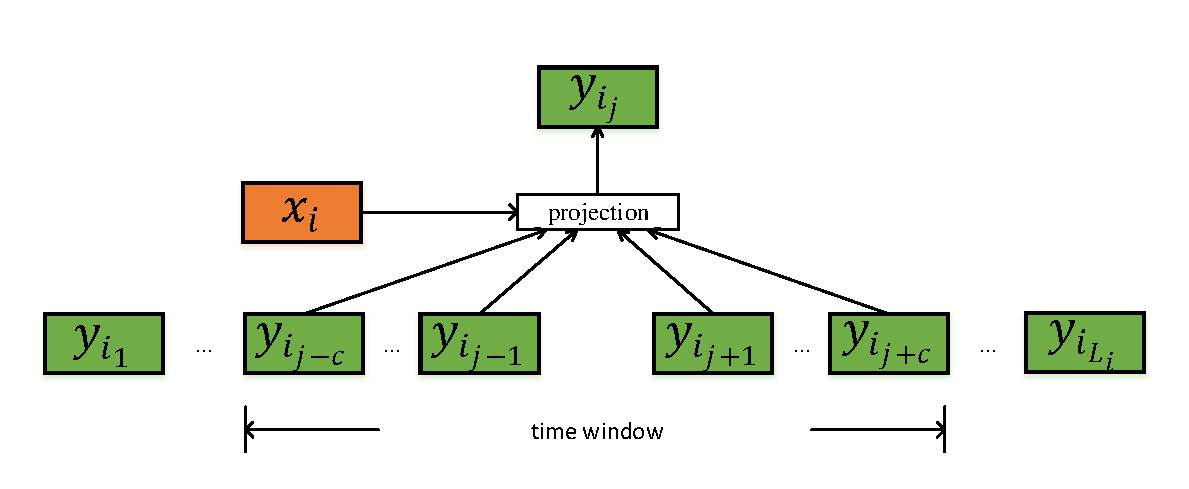
\includegraphics[scale=0.6]{images/doc2vec2.pdf}
    \caption{LSIM模型中的电影生成}
    \label{fig:doc2vec2}
\end{figure}

紧接着,我们进行观影时间线上每一部电影的生成,因为电影的生成不仅取决于用户的长期兴趣还取决于较短时间区间内的短期兴趣,
所以我们使用大小为$c$的滑动窗口规范出一个较短的时间区间用以生成当前电影,其过程如图\ref{fig:doc2vec2}所示。
从图中可以看到,一部电影的生成受到用户输入向量和同一滑动窗口内的邻居电影的影响,具体公式为:

\begin{equation}
p(y_{i_j} | y_{i_{j-c}} : y_{i_{j+c}}, x_i) =
\frac
{
    exp( \overline{\mathbf{v}}_{2}^{\mathrm{T}} \mathbf{v}_{y_{i_j}}^{'} )
}
{
    \sum_{y^{'}} exp( \overline{\mathbf{v}}_{2}^{\mathrm{T}} \mathbf{v}_{y^{'}}^{'} )
}
\end{equation}

其中$y^{'}$代表用户集合中的每一部电影,${y_{i_j}}$代表当前待生成的电影,
$\mathbf{v}_{y^{'}}^{'}$和$\mathbf{v}_{y_{i_j}}^{'}$是分别是它们的输出向量表示,
整个公式的含义就是在当前用户和邻居电影的前提下,待生成电影的生成概率要大于其他电影的生成概率,
而$\overline{\mathbf{v}}_{2}$是同一个短期兴趣窗口内邻居电影的向量表示的平均值,即
\begin{equation}
\overline{\mathbf{v}}_{2} = \frac{
    \mathbf{v}_{x_i} + 
    \sum_{-c \leq k \leq c, k \not= 0}{\mathbf{v}_{y_{i_{j+k}}}}
}{2c+1}
\end{equation}

\subsubsection{整体生成}
了解完用户生成和电影生成之后,最后我们将两者进行合并作为对输入样本的整体生成,即对于每一个观影时间线的输入,
最大化用户生成和各部电影生成的概率和,那么对于整个训练集的观影时间线的所有输入,
我们最大化所有训练样本上整体生成概率之和,具体公式为:

\begin{equation}
\sum_{i=1}^{N} \bigg( p(x_i | y_{i_1}, y_{i_2}, ..., y_{i_{L_i}}) +
\sum_{j=1}^{L_i} p(y_{i_j} | y_{i_{j-c}} : y_{i_{j+c}}, x_i) \bigg)
\end{equation}

初始状态下,本文首先将用户嵌入向量和电影嵌入向量随机初始化为一个长度为$K$的数值向量,然后通过训练过程中的误差反向传播对其进行更新,
通过若干轮训练集合的输入迭代,即可更新出包含丰富序列信息的用户嵌入表示和电影嵌入表示。
本文采用随机梯度下降(Stochastic Gradient Descent, SGD)对优化目标进行迭代求解,
同时层次Softmax(Hierarchical Softmax)和负采样(Negative Sampling)是两个常见的计算加速算法,
在本文中,我们使用负采样的方法进行计算加速。

\subsection{电影评分生成}
长短期兴趣模型并不能直接预测出缺失的电影评分,而是得到包含序列信息的用户嵌入表示和电影嵌入表示,
为了通过两种表示最终生成待预测的电影评分,我们需要引入基于特征的协同过滤框架。
基于特征的矩阵分解由chen等人\parencite{chen2011feature}在2011年提出,是矩阵分解算法的一个变种,和传统的矩阵分解不同的是,
它允许我们在创建分解模型的同时利用诸多辅助信息,例如用户画像,物品属性,好友关系和时间动态等等。

\begin{figure}[htbp]
    \centering
    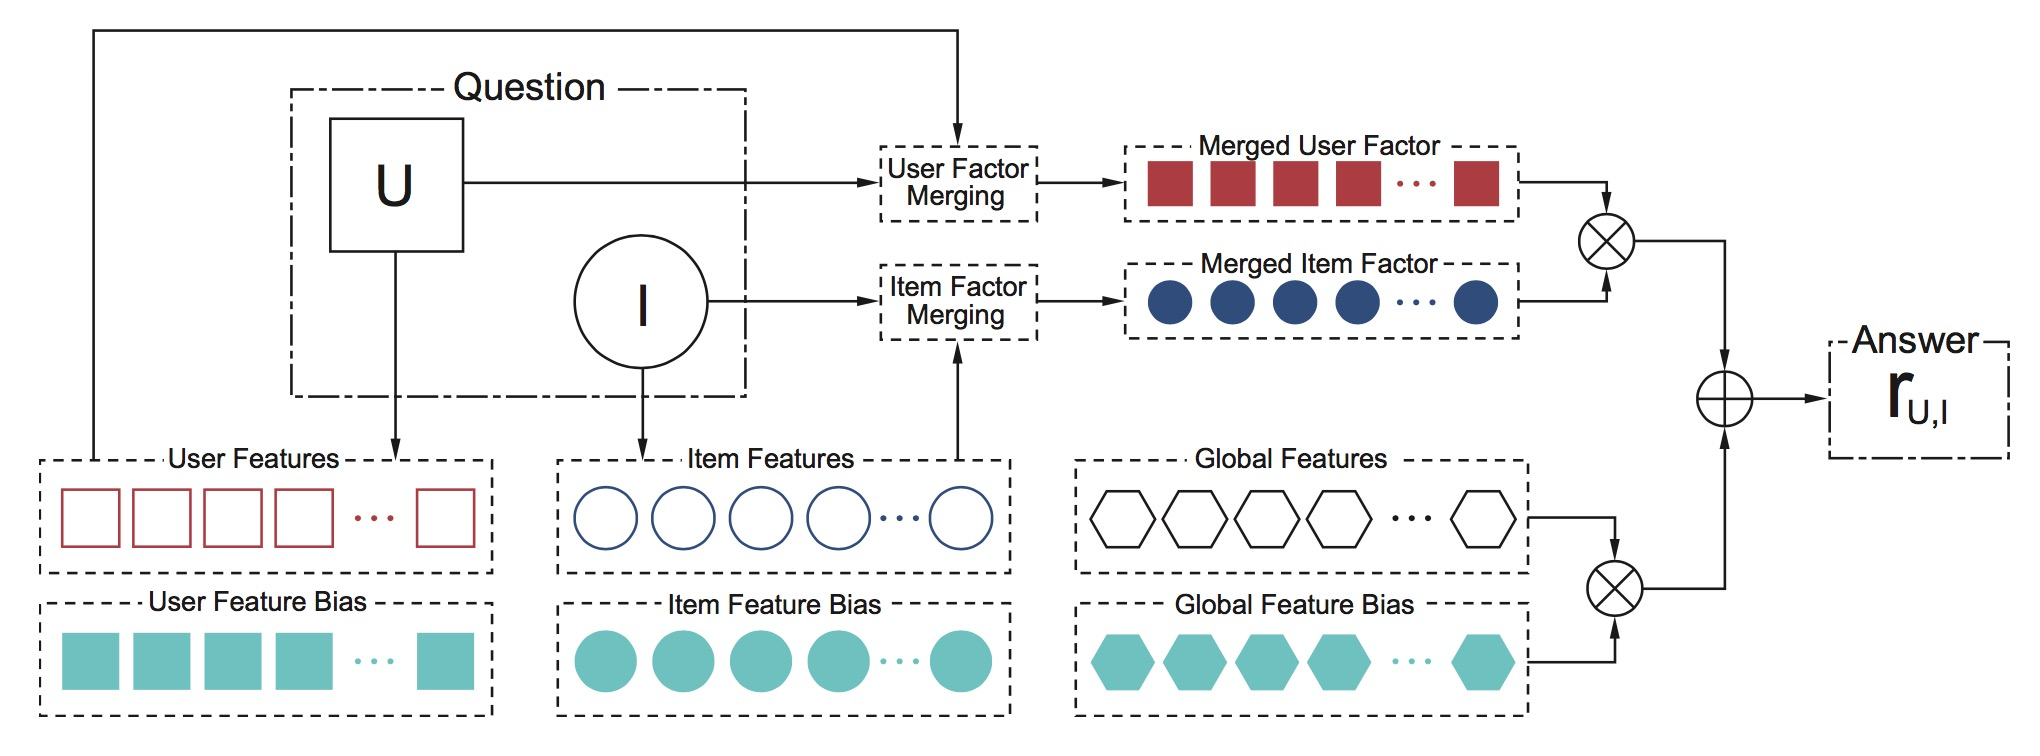
\includegraphics[scale=0.22]{images/svdfeature.jpeg}
    \caption{基于特征的矩阵分解}
    \label{fig:svdfeature}
\end{figure}

基于特征的矩阵分解框架如图\ref{fig:svdfeature}所示,从图中我们可以观察得到,特征一共可以分为三类:用户特征、物品特征和全局特征。
Question,也就是框架的输入,包含用户ID和物品ID,Answer,也就是框架的输出,对应到用户给定该物品的评分数值。
在框架中,首先会通过用户ID和物品ID找到对应的用户特征和物品特征,合并之后形成用户因子向量和物品因子向量,即图中的红色方块和蓝色圆圈,
然后将用户因子向量和物品因子向量进行交互处理,紧接着再加上全局特征的影响,最终得到待预测的评分。

为了方便和别的算法进行对比,本文只考虑了用户特征和物品特征,没有使用全局特征。我们使用$\mathbf{u}_i \in \mathbb{R}^{n}$代表用户特征,
$\mathbf{v}_j \in \mathbb{R}^{m}$代表物品特征,那么基于特征的矩阵分解所得到的预测评分数值$\hat{r}$的公式为

\begin{equation}
\hat{r}_{ij} = \sum_{k=1}^{n} \alpha_k \mathbf{u}_{ik} + \sum_{k=1}^{m} \beta_k \mathbf{v}_{jk} +
\left( \sum_{k=1}^{n} \mathbf{u}_{ik} \mathbf{p}_k \right) ^ \mathrm{T}
\left( \sum_{k=1}^{m} \mathbf{v}_{jk} \mathbf{q}_k \right)
\end{equation}

其中$\alpha$和$\beta$分别控制着用户特征和物品特征的影响程度
$\mathbf{p}_{k} \in \mathbb{R}^K$和$\mathbf{q}_{k} \in \mathbb{R}^K$
是$K$维的和每一个特征相关的隐向量因子。如果我们使用独热向量(One-Hot Representation)来表示用户和物品,即

\begin{equation}
\mathbf{u}_{ik} =
\left\{
\begin{aligned}
1, &\quad k = i \\
0, &\quad k \not= i
\end{aligned}
\right. \\ , \quad
\mathbf{v}_{jk} =
\left\{
\begin{aligned}
1, &\quad k = j \\
0, &\quad k \not= j
\end{aligned}
\right. \\
\end{equation}

那么上文中的评分预测公式就会退化为基本的矩阵分解算法,
即
\begin{equation}
\hat{r}_{ij} = \alpha_i + \beta_j + \mathbf{p}_i ^ \mathrm{T} \mathbf{q}_j
\end{equation}

其中$\alpha$和$\beta$分别代表用户偏移和物品偏移,
而$\mathbf{p}_i$和$\mathbf{q}_j$分别代表用户$\mathbf{u}_i$和物品$\mathbf{v}_j$
对应的隐向量因子。

在本文的工作中,我们使用长短期兴趣模型中学习出来的用户表示和物品作为一种辅助信息。
因此,我们定义$\tilde{\mathbf{u}}_i$代表学习出来的用户表示,
$\tilde{\mathbf{v}}_j$代表学习出来的物品表示。
然后,我们通过组合学习出的用户物品表示和经典的独热表示得到新的特征组合,即

\begin{equation}
\mathbf{u}_{i} = \{ \mathbf{u}_{i} , \tilde{\mathbf{u}}_i \} , \quad
\mathbf{v}_{j} = \{ \mathbf{v}_{j} , \tilde{\mathbf{v}}_j \}
\end{equation}

因此评分预测的公式将会变为

\begin{equation}
\begin{aligned}
\hat{r}_{ij} =
&\sum_{k=1}^{N+D} \alpha_k \{ \mathbf{u}_i , \tilde{\mathbf{u}}_i \}_k +
\sum_{k=1}^{M+D} \beta_k  \{ \mathbf{v}_j , \tilde{\mathbf{v}}_j \}_k + 
&\left( \sum_{k=1}^{N+D} \{ \mathbf{u}_i , \tilde{\mathbf{u}}_i \}_k \mathbf{p}_k \right) ^ \mathrm{T}
\left( \sum_{k=1}^{M+D} \{ \mathbf{v}_j , \tilde{\mathbf{v}}_j \}_k \mathbf{q}_k \right)
\end{aligned}
\end{equation}

其中$N$是推荐系统中的用户的数量,$M$是推荐系统中物品的数量,
$D$本文提出的长短期兴趣模型中学习出来的用户特征和物品特征的维度,
$\mathbf{p}_{k} \in \mathbb{R}^K$和$\mathbf{q}_{k} \in \mathbb{R}^K$
是$K$关联到每个特征的隐向量因子的维度。




